% =====================================================================
% Extended Data figures — Nature Human Behaviour submission
% Compile: pdflatex extended_data_NHB.tex (twice). Figures in ./figures/
% Extended Data: <=10 display items; legends also go in the Inventory of
% Supporting Information. Each item is cited as a discrete item in the main text.
% =====================================================================
\documentclass[11pt]{article}
\usepackage[margin=1in]{geometry}
\usepackage[T1]{fontenc}
\usepackage[utf8]{inputenc}
\usepackage{mathptmx}
\usepackage{graphicx}
\usepackage{caption}
\DeclareCaptionLabelSeparator{pipe}{\ \textbar\ }
\captionsetup[figure]{name=Extended Data Fig., labelsep=pipe, font=small,
  labelfont=bf, singlelinecheck=false, justification=raggedright, skip=3pt}
\usepackage[colorlinks=true,urlcolor=blue]{hyperref}
\newcommand{\supfig}[1]{Supplementary Fig.~#1}

\begin{document}

\begin{center}
{\Large\bfseries Extended Data Figures}\\[2pt]
{\small Robust but scale-dependent digital phenotypes of mental disorders}
\end{center}

\begin{figure}[htbp]\centering
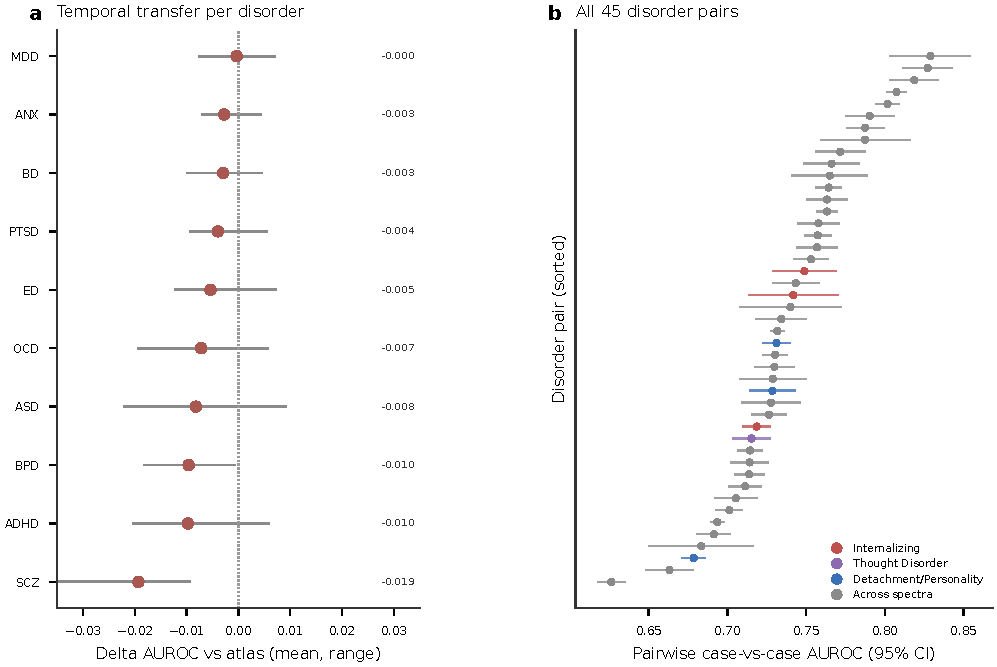
\includegraphics[width=\linewidth]{figures/ed1_validity_detail_lyc.pdf}
\caption{\textbf{Validity detail: temporal transfer and pairwise separability.}
\textbf{a}, Temporal transfer per disorder: mean $\Delta$AUROC versus the 93-feature atlas
across the three era pairs (dot), with the range (line). \textbf{b}, All 45 pairwise
case-versus-case AUROCs with 95\% confidence interval, sorted, coloured by HiTOP spectrum
(grey, across spectra).}
\label{fig:ed1}
\end{figure}

\begin{figure}[htbp]\centering
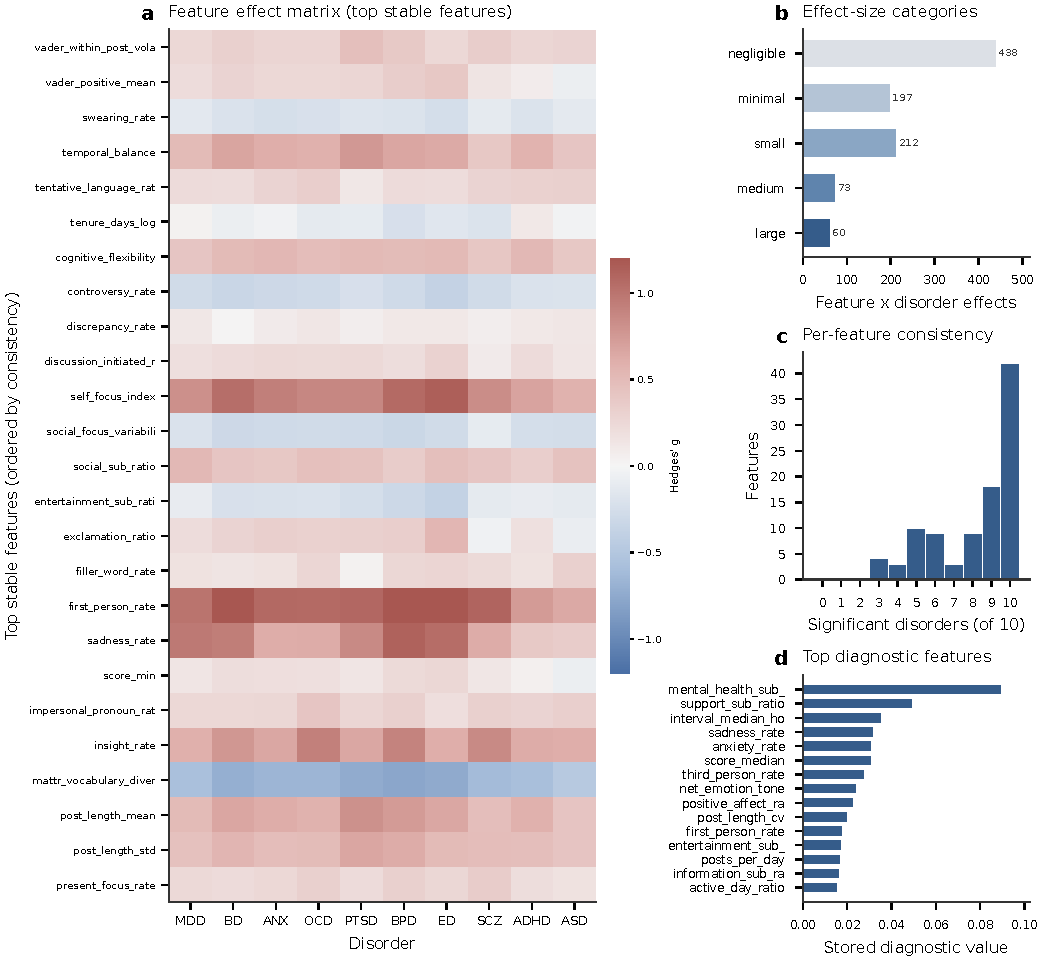
\includegraphics[width=\linewidth]{figures/ed2_feature_robustness_lyc.pdf}
\caption{\textbf{Feature-level robustness.} \textbf{a}, Feature $\times$ disorder effect-size
matrix for the 25 most consistent features (ordered by the number of significant disorders;
colour, Hedges' $g$). \textbf{b}, Counts of feature $\times$ disorder effects by effect-size
category. \textbf{c}, Per-feature consistency: number of disorders with a significant
global-false-discovery-rate effect. \textbf{d}, Top 15 features by stored diagnostic value.}
\label{fig:ed2}
\end{figure}

\begin{figure}[htbp]\centering
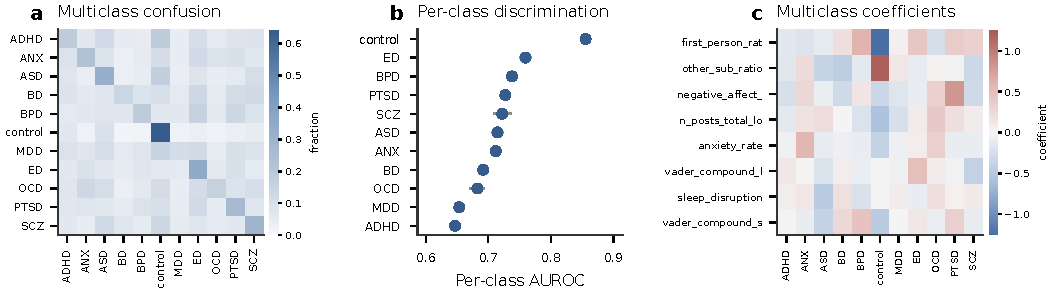
\includegraphics[width=\linewidth]{figures/ed3_discrimination_detail_lyc.pdf}
\caption{\textbf{Discrimination detail.} \textbf{a}, Normalised multiclass confusion matrix
(ten disorders and a comparison class). \textbf{b}, Per-class AUROC (mean, s.d.). \textbf{c},
Multiclass coefficients for the eight highest-loading features across classes.}
\label{fig:ed3}
\end{figure}

\begin{figure}[htbp]\centering
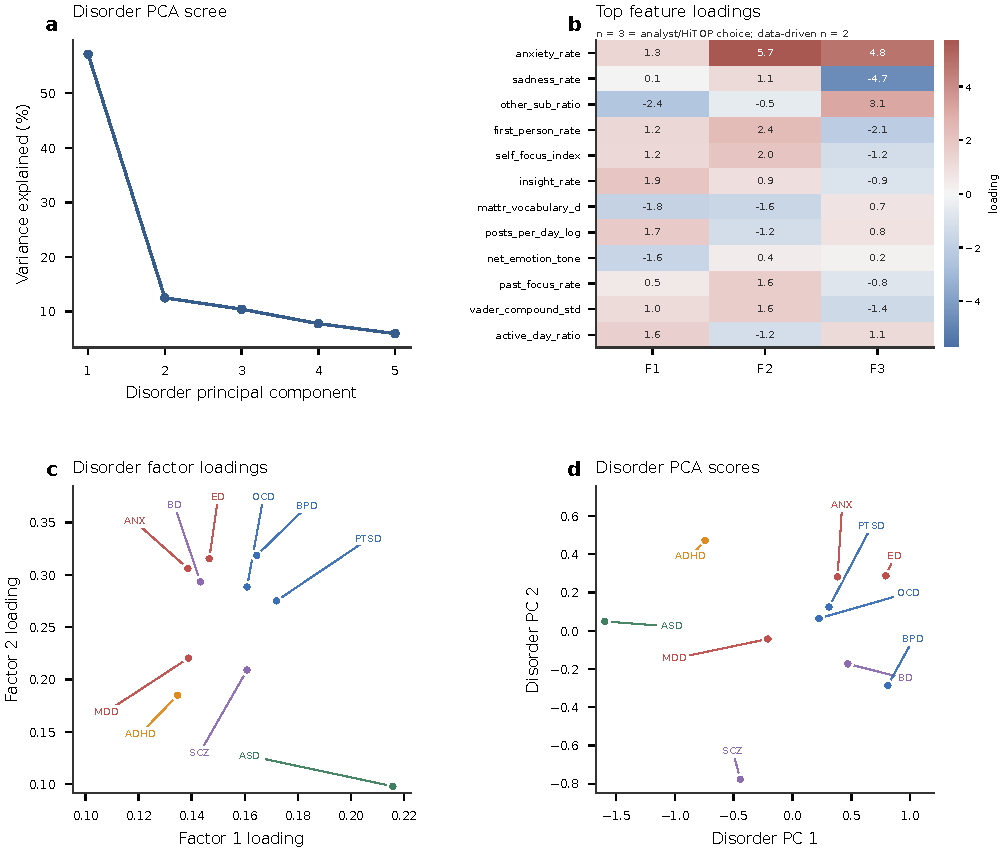
\includegraphics[width=\linewidth]{figures/ed4_factor_robustness_lyc.pdf}
\caption{\textbf{Factor and component robustness.} \textbf{a}, Disorder-level
principal-component-analysis scree plot. \textbf{b}, Loadings of the 12 highest-loading
features on the three retained factors. \textbf{c}, Disorder positions on the first two
factors of the three-factor solution. \textbf{d}, Disorder positions on the first two
disorder-level principal components.}
\label{fig:ed4}
\end{figure}

\begin{figure}[htbp]\centering
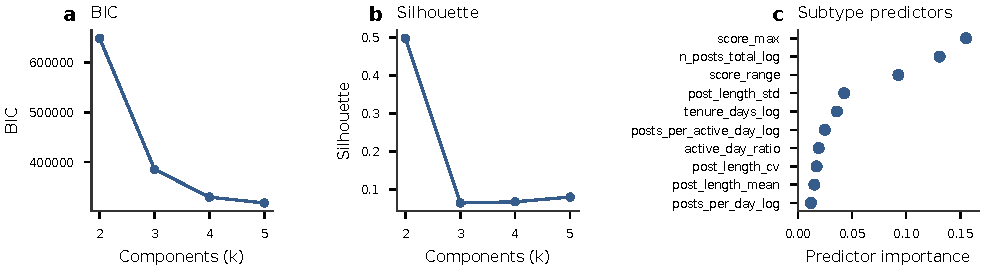
\includegraphics[width=\linewidth]{figures/ed5_gmm_detail_lyc.pdf}
\caption{\textbf{Gaussian-mixture detail.} \textbf{a}, Bayesian information criterion versus
the number of components $k$. \textbf{b}, Silhouette versus $k$ ($k=2$ was retained: the model
code starts from the Bayesian-information-criterion minimum, $k=5$, and falls back to the
smallest $k$ whose silhouette reaches 0.15; only $k=2$ qualifies, so $k=2$ is selected because
silhouette vetoes $k\ge3$, not because Bayesian information criterion supports it).
\textbf{c}, Top ten subtype predictors (importance, mean, s.d.). Stability (reported here
because the corresponding panel was merged into this legend): the subtype solution agrees
across initialisation seeds (adjusted Rand index 0.999) and is moderately stable under
bootstrap resampling (adjusted Rand index 0.70 $\pm$ 0.04, $n=30$).}
\label{fig:ed5}
\end{figure}

\begin{figure}[htbp]\centering
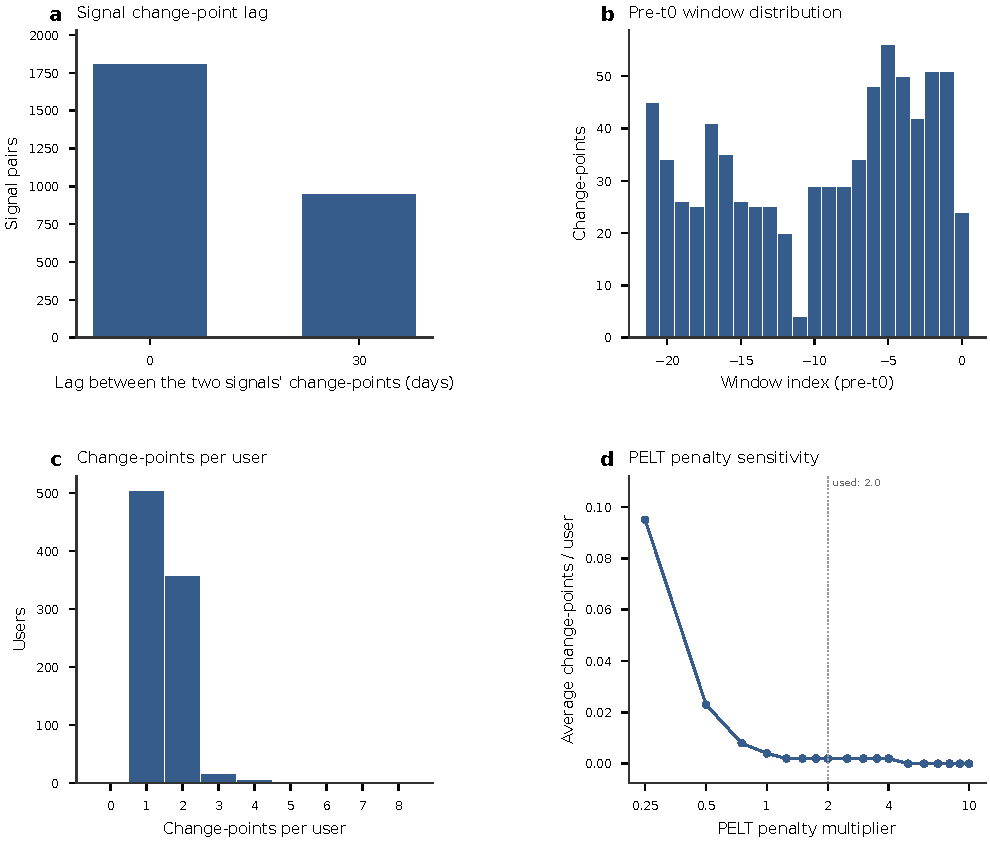
\includegraphics[width=\linewidth]{figures/ed6_trajectory_detail_lyc.pdf}
\caption{\textbf{Trajectory detail.} \textbf{a}, Lag between the change-points of the two
signals compared in the multivariate change-point analysis (values on the 30-day window grid).
\textbf{b}, Distribution of the pre-diagnosis change-point window index. \textbf{c}, Number of
change-points per user (one row per user; users with $\ge$1 change-point only). \textbf{d},
Sensitivity of the mean number of change-points per user, averaged over all users, to the
change-point penalty multiplier (log scale); dotted line, multiplier used in the main analysis
(2.0). Panels \textbf{c} and \textbf{d} use different denominators: \textbf{c} counts
change-points per affected user, whereas \textbf{d} averages over all users.}
\label{fig:ed6}
\end{figure}

\begin{figure}[htbp]\centering
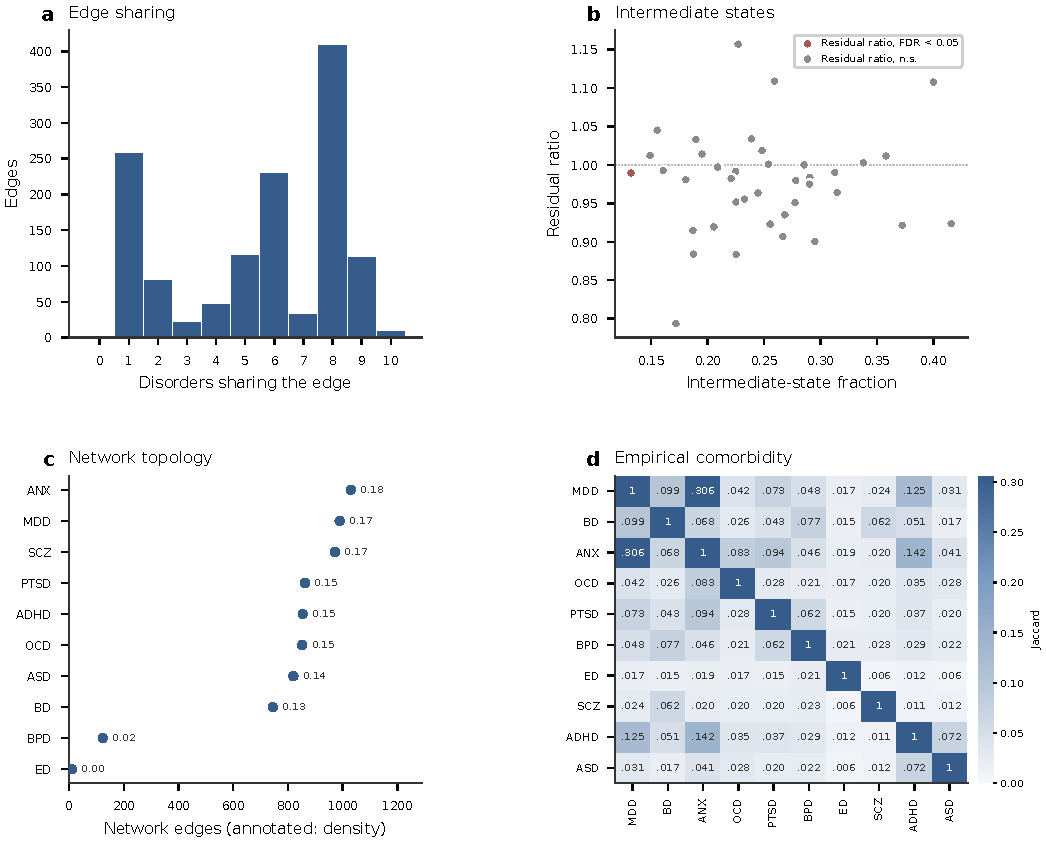
\includegraphics[width=\linewidth]{figures/ed7_network_detail_lyc.pdf}
\caption{\textbf{Network and intermediate-state detail.} \textbf{a}, Number of disorders
sharing each feature edge. \textbf{b}, Intermediate-state fraction against the residual ratio
(dual-state residual relative to the reference residual), coloured by the false-discovery-rate
of the residual-ratio Mann--Whitney test; dotted line, ratio of 1. \textbf{c}, Network topology
per disorder: number of edges (density annotated). \textbf{d}, Empirical (cohort-overlap)
comorbidity matrix (Jaccard).}
\label{fig:ed7}
\end{figure}

\begin{figure}[htbp]\centering
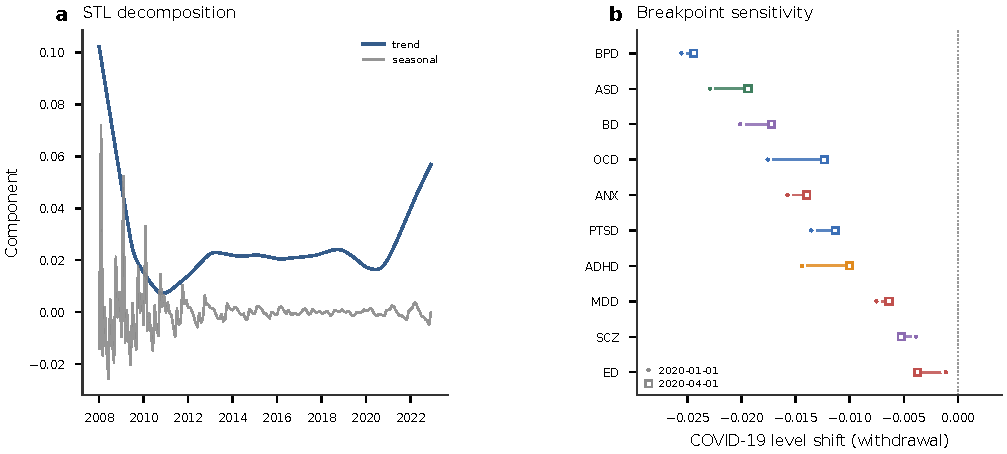
\includegraphics[width=\linewidth]{figures/ed8_population_detail_lyc.pdf}
\caption{\textbf{Population detail.} \textbf{a}, Seasonal-trend decomposition using LOESS
(STL) of the pooled digital signal: trend and seasonal components (monthly, 179 months).
\textbf{b}, Breakpoint sensitivity of the COVID-19 level shift (withdrawal signal): closed
circle, breakpoint 2020-01-01; open square, 2020-04-01; one row per disorder.}
\label{fig:ed8}
\end{figure}

\begin{figure}[htbp]\centering
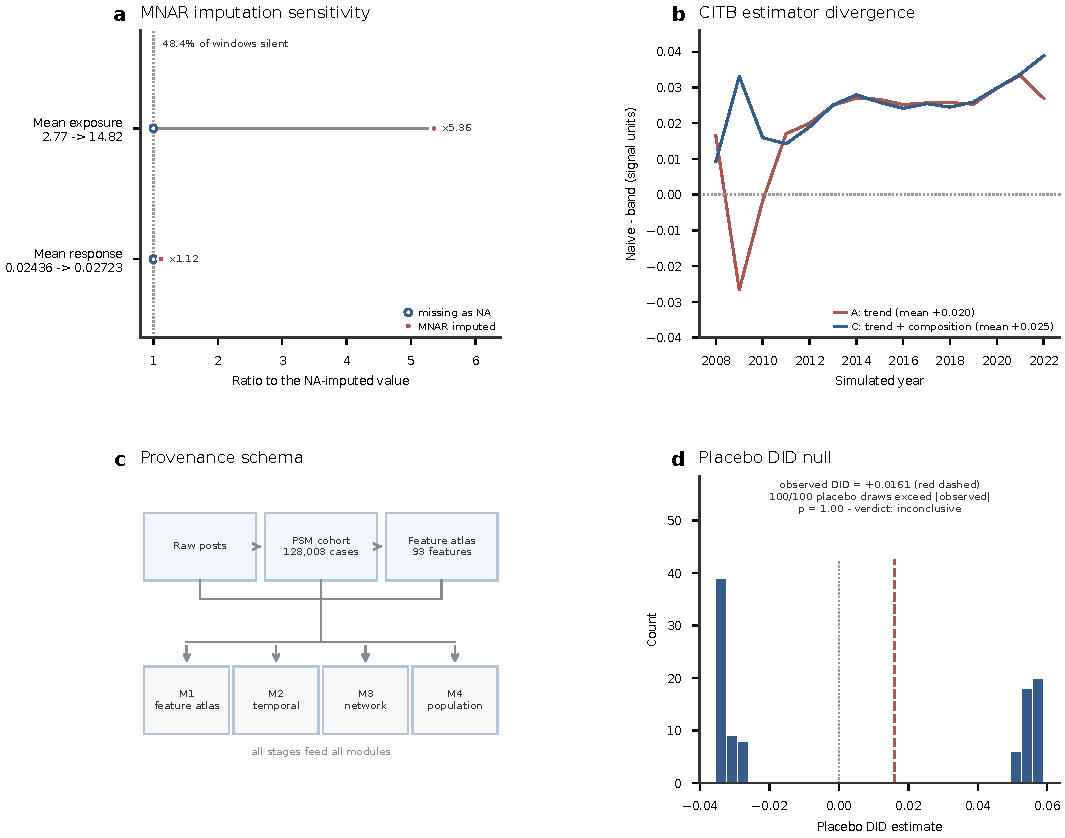
\includegraphics[width=\linewidth]{figures/ed9_assumptions_provenance_lyc.pdf}
\caption{\textbf{Assumptions and provenance.} \textbf{a}, Missing-not-at-random silent-window
imputation sensitivity: ratio of the imputed to the missing-as-NA aggregate for mean exposure
and mean response. \textbf{b}, Estimator divergence for scenarios A and C (naive minus
band-adjusted recovered series). \textbf{c}, Data-provenance schema: the construction pipeline
feeds all four analysis modules. \textbf{d}, Placebo difference-in-differences draw
distribution (100 draws) with the observed difference-in-differences (the stored placebo
outcome was inconclusive, $P=1.0$).}
\label{fig:ed9}
\end{figure}

\begin{figure}[htbp]\centering
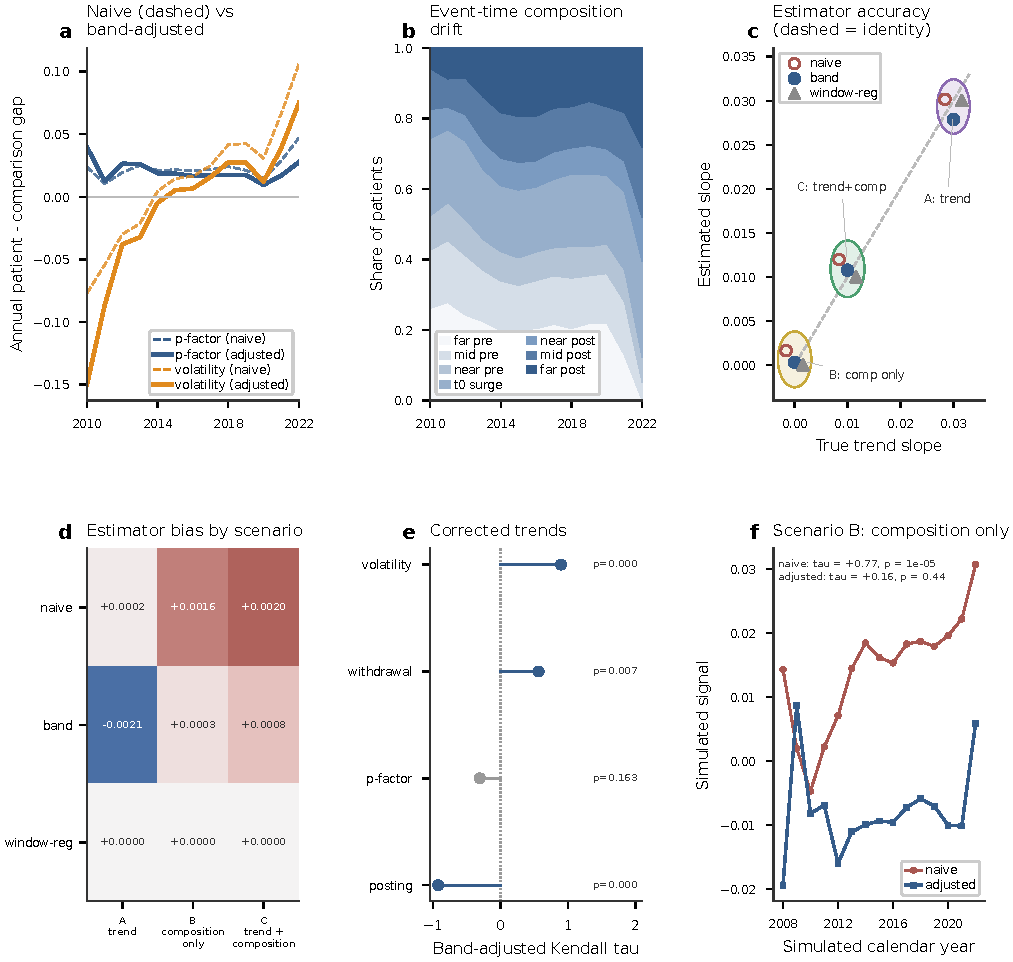
\includegraphics[width=\linewidth]{figures/ed10_citb_audit.pdf}
\caption{\textbf{Composition-induced temporal bias (CITB) audit.} \textbf{a}, Calendar-time
case-minus-comparison gap, naive (dashed) versus event-time band-adjusted (solid), for the
p-factor and volatility signals, 2010--2022. \textbf{b}, Stacked area of the event-time band
composition (share of diagnosed users per band) by calendar year. \textbf{c}, Estimated versus true
trend slope for three estimators (naive, band-adjusted and window regression) across three
scenarios (A, trend; B, composition only; C, trend plus composition); dashed line, identity.
\textbf{d}, Estimator bias (slope minus true trend) by scenario, on a zero-centred diverging
scale. \textbf{e}, Band-adjusted Kendall $\tau$ per signal (grey, $P\ge0.05$; blue,
$P<0.05$), with $P$ values at right. \textbf{f}, Simulated scenario B (composition only, no
true trend): naive versus band-adjusted series, with the stored Kendall trend statistics
annotated.}
\label{fig:ed10}
\end{figure}

\end{document}